\documentclass[10pt,a4paper]{article}
\usepackage[a4paper, left=3cm, right=3cm, top=3cm, bottom=3cm, headsep=10mm, footskip=12mm]{geometry}
\usepackage[T1]{fontenc}
\usepackage[ngerman, english]{babel}    % mehrsprachiger Textsatz
% babel: letzte Sprache in Optionen zeigt die Sprache des Dokumentes
% und kann durch den Befehl \selectlanguage{} geaendert werden
% Passen Sie die Optionen des babel-Paketes nach Bedarf an!
\usepackage{float}
\usepackage{graphicx}
\usepackage{url}
\usepackage{pdflscape}
\usepackage{mathtools}
\usepackage{amssymb, amsmath, amstext}
\usepackage{amsthm}
\usepackage{xcolor}
\usepackage{nameref}
\usepackage{siunitx}
\usepackage{makecell}
\usepackage{hyperref}
\usepackage{enumitem}
\usepackage[superscript,biblabel]{cite}
\usepackage{caption}
\usepackage{subcaption}
\usepackage{tabularx} 			% Tabellen erzeugen
\usepackage{multirow}			 % Zeilen in Tabellenbearbeitung
\usepackage{multicol} 			% Spalten in Tabellenbearbeitung 
\usepackage{lmodern}                        % Ersatz fuer Computer Modern-Schriften 
\usepackage{amsmath}                                           % zum besseren Aussehen am Bildschirm
\usepackage{booktabs} % für schönere Tabellen
\usepackage{sidecap}
\usepackage{rotating} % für die Landscape-Umgebung
\usepackage{afterpage}
\definecolor{Bluetitle}{HTML}{1F3864}
\definecolor{softbluetitle}{HTML}{274D7E}
\definecolor{Greyish}{HTML}{5A5A5A}
\renewcommand{\refname}{Reference}
\usepackage{array,multirow}
%\newcommand{\specialcell}[2][c]{%\begin{tabular}[#1]{@{}c@{}}#2\end{tabular}}




\begin{document}
	
	\begin{titlepage}
		\begin{center}
			\begin{figure}[h!tbp]
				
\includegraphics[width=\linewidth]{HUlogo.PNG}
			\end{figure}
			\vspace*{2 cm}
			
			\textcolor{Bluetitle}{\textbf{\huge Infrarotspektroskopie}}\par
			\vspace*{0.5cm}
			\textcolor{softbluetitle}{\textbf{\Large ATR und Transmissionsspektroskopie}}\par
			
			\vspace*{2cm}
			
			\textcolor{Greyish}{\textbf{Versuchsdurchführende}}\par
			\textcolor{Greyish}{Tom Oberländer (633676)}\par
			\textcolor{Greyish}{Huyen Anh Nguyen (572309)}\par
			
			\vspace*{0.5cm}
			\textcolor{Greyish}{\textbf{Versuchsort}}\par
			\textcolor{Greyish}{Invalidenstraße 42, Erdgeschoss rechts}\par
			\textcolor{Greyish}{Institut für Biophysik}\par
			\vspace*{0.5cm}
			\textcolor{Greyish}{\textbf{Versuchsbetreuer}}\par
			\textcolor{Greyish}{Prof. Dr. Franz Bartl}\par
			
			\vspace*{2 cm}
			
			\textcolor{Greyish}{5. Juli 2024}\par
			
			
			
			
		\end{center}
	\end{titlepage}
	
	\tableofcontents
	
	\section{Einführung}	
	Anders als in der klassischen Spektroskopie wird in der Infrarot (abgekürzt:IR) - Spektroskopie nicht die Änderung der Energiezustandes der Elektronen in der äußersten Schalen der Probe untersucht, sondern die Änderung der Schwingungszustandes des Moleküles.\\
	Die Energie, die ein Molekül bzw Atom von den IR-Strahlungen absorbiert, reicht aus um die Rotationszustandes eines Moleküls und der Schwingungszustandes einer Bindung charakteristisch zu verändern.
	Dadurch ist es möglich die Struktur eines Moleküles zu untersuchen.\\
	\\
	In der IR-Spektroskopie gibt es unterschiedliche Methoden, wie die IR-Wellen genutzt werden kann um die Proben zu untersuchen.\\
	Der Klassiker in der Spektroskopie ist die Transmissionsspektroskopie.\\
	Dort wird die Probe mit IR-Strahlung bestrahlt und die durchgegangene Strahlung am Detektor gemessen.
	Je nach dem wie IR-aktiv ein Stoff ist, wird mehr oder weniger absorbiert, wodurch dann ein IR-Absorptionsspektrum gemessen werden kann.
	Bei den Proteinen gibt es neun verschiedene IR-aktive Schwingungen, die in bestimmten Wellenzahlintervallen (Absortionsbanden) liegen. Die Banden werden als Amid A,B, I bis VII - Bande bezeichnet.\\
	Für die Sekundärstrukturaufklärung in Proteinen ist die Amid I Bande am wichtigsten, da diese zum größtenteils durch die C=O Streckschwingung der Peptidbindung verursacht wird. Die Amid I Bande ist ein Komposition aus C=O - Valenzschwingungen, C-N-Streckschwingungen und N-H-Deformationsschwingungen, die in den Bereich 1600-1700 cm$^{-1}$ liegen.
	Aufgrund dieser IR-Aktivität der Peptidbindung, kann die Sekundärstruktur von Polylysin bei den Bedingung :
	\begin{itemize}
		\item neutralen pH und auf Eis
		\item basischen pH und auf eis
		\item basischen pH und auf 50°C erhitzt
	\end{itemize}
	untersucht werden.\\
	\\
	Eine andere Messmethode in der IR-Spektroskopie ist die attenuated total Reflexion (abgekürzt: ATR) - Spektroskopie.
	Hier wird die Probe auf ein Kristall (Zinksilicium-Kristallzelle) aufgetragen und die IR-Strahlungen so auf das Kristall bestrahlt, so dass eine Totalreflexion im Kristall entsteht. Dabei bildet sich an der Grenzfläche eine evaneszente Welle, die mit der Probe interagieren kann. Durch die Interaktion wird die Intensität der reflektierte IR-Strahlung abgeschwächt\cite{ATR_wiki}.
	Die Intensität der reflektierten IR-Strahlung ist ebenfalls von der Probe abhängig, wodurch dieses Messprinzip verwendet werden kann, um feste aber auch flüssige Proben, wie die Citronensäure, zu charakterisieren.
	Ein Vorteil dieser Methode ist, dass die Messung unabhängig von der Probemenge \cite{ATR_MT} ist.


	\section{Material und Methode}
	Alle Messungen wurden am IFS 66v/S Spektrometer (Bruker, Berlin - Humboldt Universität zu Berlin am Biophysik Institut) durchgeführt.\\
	Auf die ATR-Zelle (Zinksilicium-Kristall) wurde so viel Wasser und Deuteriumoxid raufpipettiert, bis dieser vollständig bedeckt war und davon ein Infrarotspektrum jeweils aufgenommen.\\
	Für die Konzentrationsbestimmung der Proben wurde ein linearen Fit mit der Funktion curve$\_$fit (scipy, Python) durchgeführt.\\
	
		\subsection{Citronensäure-Messungen}
		Die Citronensäureproben wurden in Wasser gelöst und bei Normaldruck und 20 Grad Celsius auf die ATR-Zelle aufgetragen und das IR-Spektrum gemessen.\\
		Das Gleiche wurde für die Verdünnungsreihe (Pipettierschema siehe Table: \ref{fig:IR_Standardcurve}) durchgeführt.\\
		Um Hintergrundsrauschen zu minimieren, wurde die Luft im Messgerät geblankt.\\
		
	
		\subsection{Polylysin}
		Polylysin (grob 10 mg/mL) wurde in Deuteriumoxid gelöst und das Transmissionsspektrum im Vakuum bei 20 Grad Celcius gemessen.\\
		Die Proben wurden vor der Messung vorher in drei unterschiedlichen Bedingungen vorbehandelt:
		\begin{itemize}
			\item bei neutralen pH-Wert auf Eis
			\item bei pH = 11.62 (pH-Einstellung mit Natronlauge)
			\item 3 Minuten mit einer Heißluftpistole aufheizen
		\end{itemize}
		Als Blanklösung wurde Deuteriumoxid verwendet.
	
	
	
	\section{Ergebnis}
		\subsection{Wasser und Deuteriumoxid Infrarotspektrum}

			Beide besitzen ähnliche IR-Banden im Bereich von 1500 - 1900cm$^{-1}$ und 3000 - 4000  cm$^{-1}$  auf. Deuteriumoxid besitzt noch zwei weitere Banden bei 100 - 1500 cm$^{-1}$ und 2400 - 2800cm$^{-1}$ (siehe Figure \ref{fig:water}) .
		
			\begin{figure}[H]
				\centering
				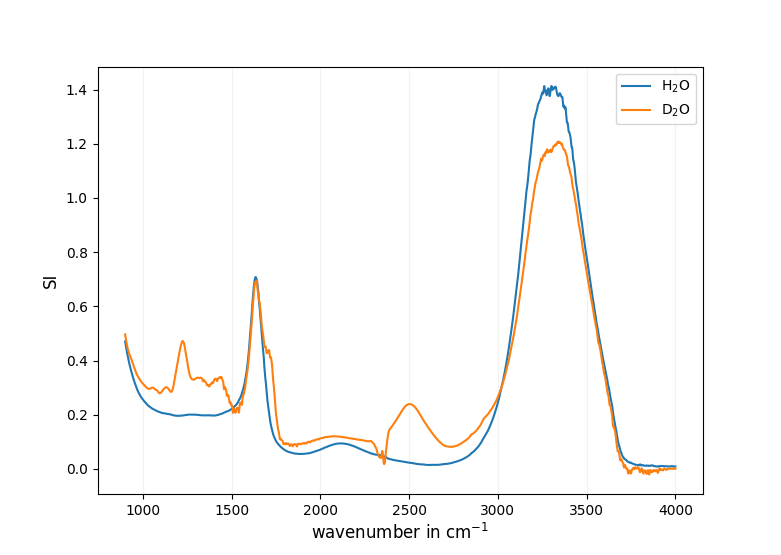
\includegraphics[scale=0.55]{Onlywater.png}
				\caption{Infrarotspektrum von Wasser.}
				\label{fig:water}
			\end{figure}
		
	
		\subsection{Charakterisierung von Citronensäure}
		
			\begin{figure}[H]
				\centering
				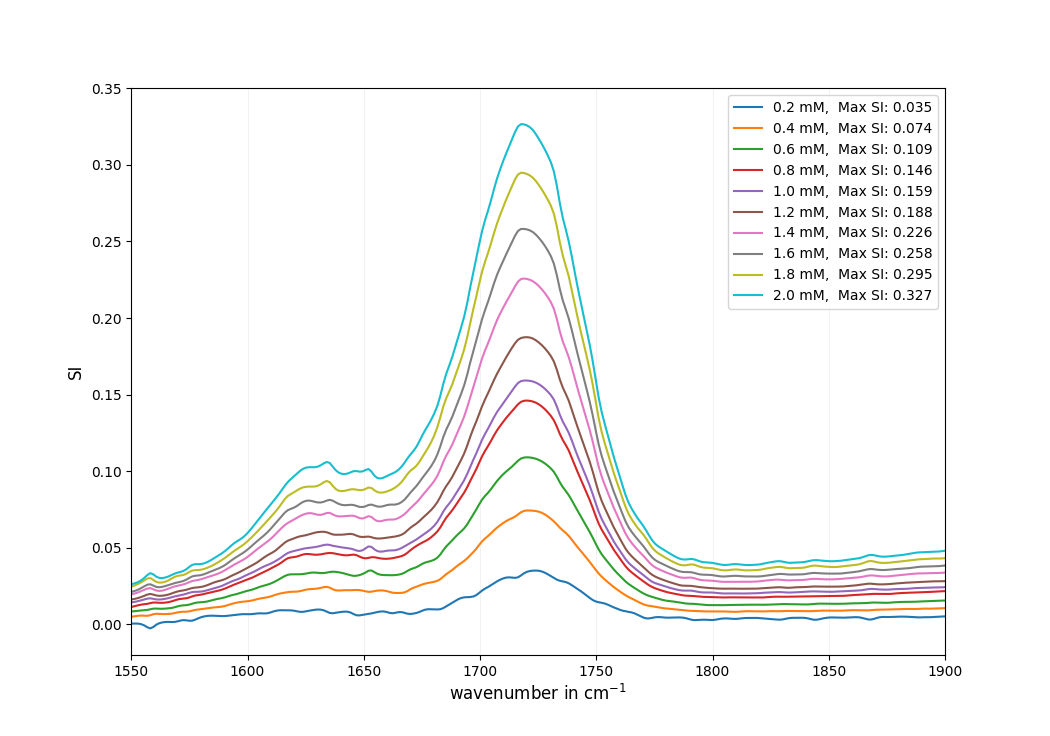
\includegraphics[scale=0.55]{Standardcurve_citricacid.png}
				\caption{Infrarotspektrum der Verdünnungsreihe von Citronensäure in Wasser. Abgebildet ist die maximale Signalintensität (SI$_{max}$) zwischen 1520 - 1900 cm$^{-1}$}
				\label{fig:IR_Standardcurve}
			\end{figure}
			
			Die SI$_{max}$ von Citronensäure liegt ungefähr im Bereich von 1718 cm$^{-1}$ und überlappt mit Wasser und Deuteriumoxid.\\

			Für die Konzentrationsbestimmung der unbekannten Proben, wurde eine Standardsreihe (oder auch Verdünnungsreihe genannt) hergestellt und gemessen.\\
			Die SI$_{max}$  der einzelnen Standardkonzentrationen wurden in Abhängigkeit der Citronensäurekonzentration aufgetragen (siehe Figure \ref{fig:Standardcurve}). a ist die Steigung der gefittete Gerade. Die Datenpunkte wurden nach der Gleichung (\ref{eq: linear_fit}) gefittet und die Konzentration der Proben (in Table \ref{tab:sampleconc}) wurden nach Gleichung (\ref{eq: concbest}) ermittelt.\\

			\begin{equation}\label{eq: linear_fit}
				SI_{max} (c)= a \cdot c\\
			\end{equation}
			
			\begin{equation}\label{eq: concbest}
				c = \frac{SI_{max}}{a}
			\end{equation}
			
			\begin{table}[H]
				\centering
				\caption{Molare Konzentration der Unbekannten Citronensäureproben berechnet aus der Standardkurve in Figure \ref{fig:Standardcurve}.}
				\label{tab:sampleconc}
				\begin{tabular}{cc}
					\toprule
					Samplename & c(Sample) in mM\\
					\midrule
					Sample 1 & 1.04 $\pm$ 0.012\\
					Sample 2 & 0.58 $\pm$ 0.007\\
					\bottomrule
				\end{tabular}
			\end{table}	

			Eine unvollständige Gauss'sche Fehlerfortpflanzung (siehe in Gleichung (\ref{eq :error}))wurde hier für die Unbekannten durchgeführt, da nicht die Messungenauigkeit des IFS 66v/S Spektrometer notiert wurde. Zudem werden auch die Fehler der Pipette vernachlässig. Der Term für die Abweichung von SI ($\Delta SI_{max}$)in der Gleichung wurde auf 0 gesetzt.
			
			\begin{equation}\label{eq :error}
				\begin{split}
					\Delta c = \sqrt{\left( \frac{SI_{max}}{a^2}\right)^2 \cdot \Delta a}
				\end{split}
			\end{equation}
			
		\begin{figure}[H]
			\centering
			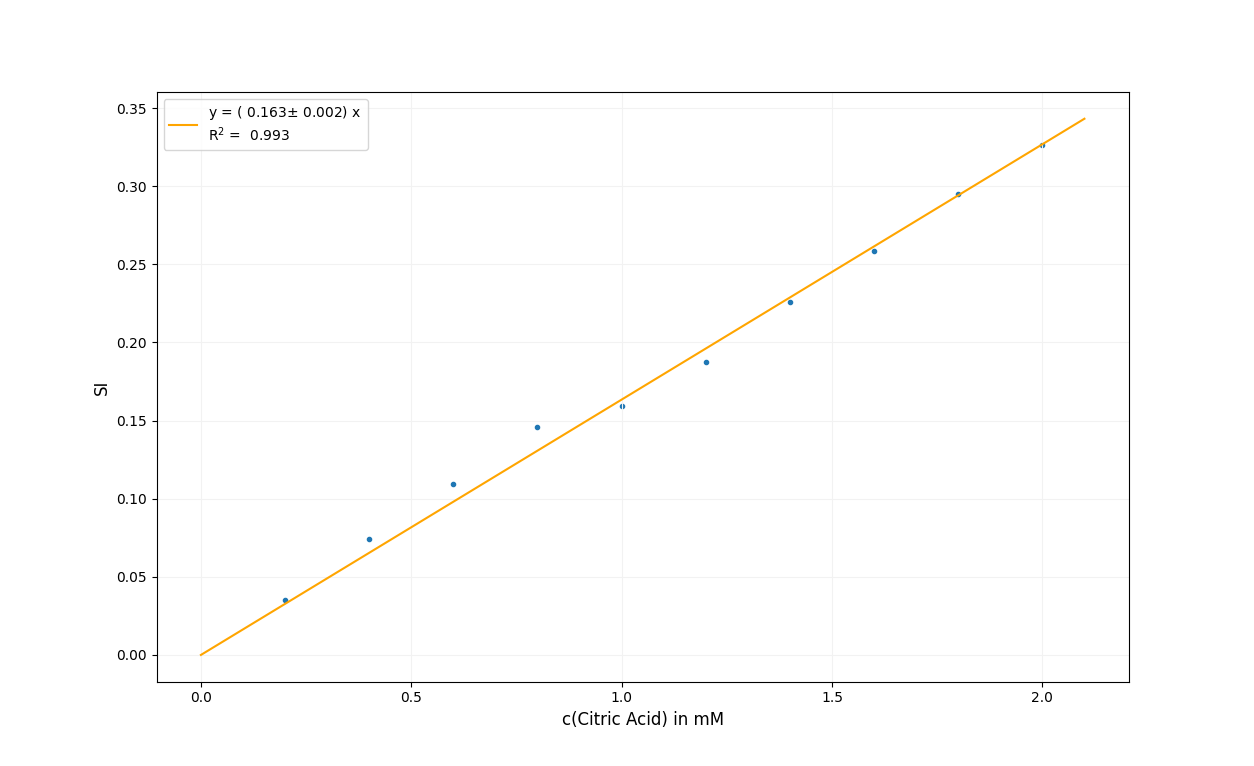
\includegraphics[scale=0.55]{Standardcurve_Fit.png}
			\caption{Standardkurve von der Citronensäure in der Abhänigkeit der maximale Signalintensität (abgekürzt: $SI_{max}$) bei $\tilde{\nu}$ = 1720 cm$^{-1}$ von Citronensäure in Wasser von der molaren Konzentration. }
			\label{fig:Standardcurve}
		\end{figure}
		

		\subsection{Sekundärstrukturanalyse von Polylysin}
		
			In Figure \ref{fig:polylysin_IR_Spektrum} wurden die drei IR-Spektrum im Wellenzahlbereich von 1560 - 1750 cm$^{-1}$ dargestellt.\\
			Polylysin zeigt bei neutralen und basischen Bedingung jeweil ein SI$_{max}$ im Bereich von circa 1640 cm$^{-1}$. Wird Polylysin auf 50 °C aufgeheißt, sind zwei SI$_{max}$ bei 1612 und 1680 cm$^{-1}$ sichtbar (siehe Table \ref{tab:Polylysin_SI}).
				
			\begin{figure}[H]
				\centering
				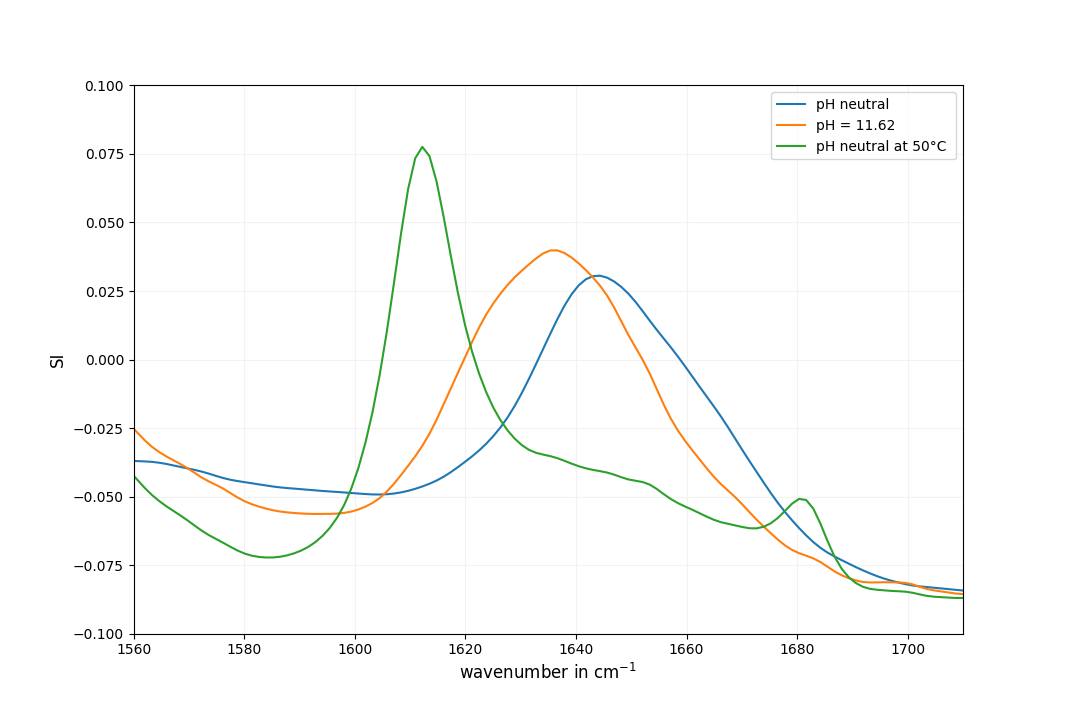
\includegraphics[scale=0.55]{Polylysin.png}
				\caption{IR-Transmissionsspektrum von Polylysin (ß $\approx$ 10 mg/mL in D$_2$O) bei unterschiedlichen Bedingungen im Wellenzahlbereich von 1560 - 1750 cm$^{-1}$.}
				\label{fig:polylysin_IR_Spektrum}
			\end{figure}
			
			\begin{table}[H]
				\centering
				\caption{Wellenzahl $\tilde{\nu}$ von Polylysin bei unterschiedlichen Bedingungen, wo im Bereich von 1560 - 1750 cm$^{-1}$ eine maximale Signalintensität zu sehen ist.}
				\label{tab:Polylysin_SI}
				\begin{tabular}{cc}
					\toprule
					Bedingung & $\tilde{\nu}_{max}$ in cm$^{-1}$\\
					\midrule
					pH neutral & 1644\\
					&\\
					pH = 11.62 & 1636\\
					&\\
					\multirow{2}{*}{50°C } & 1612\\
					& 1680\\
					\bottomrule
				\end{tabular}
			\end{table}	

	
	\section{Diskussion}
		\subsection{Wasser und Deuteriumoxid}
			In Figure \ref{fig:water} wurde das IR-Spektrum von Wasser und Deuteriumoxid dargestellt. Den Kurvenverlauf der beiden ähneln sich sehr. Bei der Datensicherung könnte eventuell ein Fehler unterlaufen sein, da Deuteriumoxid in dem Bandenbereich von Amid I der Proteine eine schwache SI$_{max}$  bei 1555 cm$^{-1}$  \cite{infrared_d2o_h2o} zeigt und eine mittelstarke SI$_{max}$  bei 1209 cm$^{-1}$  \cite{infrared_d2o_h2o}. in diesen Fall ist die SI$_{max}$ bei beiden Banden relativ gleich stark und hoch\\
			Vermutet wird, dass die in Figure \ref{fig:water} dargestellte Deuteriumoxid IR-Spektrum sich eventuell von einem Citronensäure in Wasser gelöste Probe handelt.\\
			Wird das komplette IR-Spektrum der drei Proben dargestellt, wie in Figure \ref{fig:wasser_Citrat_full}, dann sind viele Peaks ähnlich von der orangene Kurve und grüne Kurve.\\
			
			\begin{figure}[H]
				\centering
				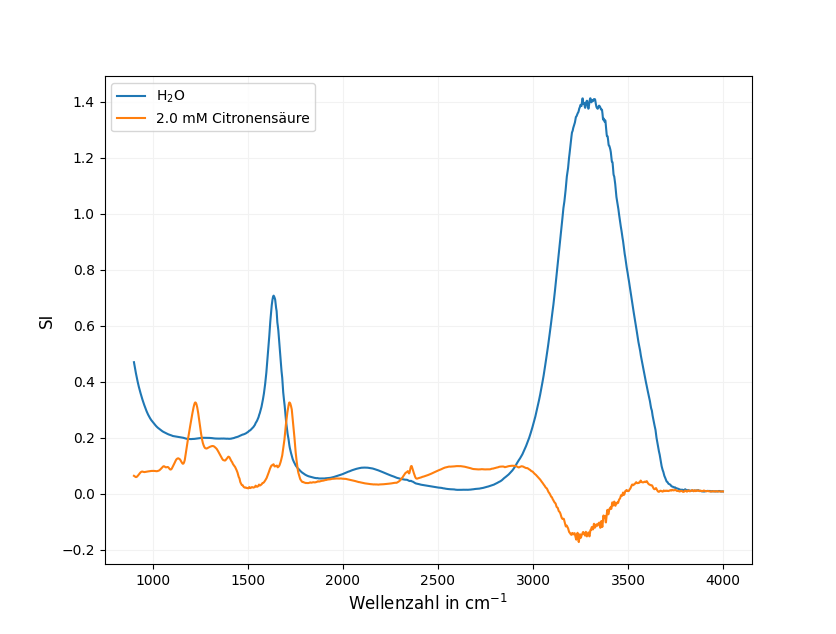
\includegraphics[scale=0.55]{water_citricacid.png}
				\caption{Infrarotspektrum von Wasser, Deuteriumoxid und 2 mM Citronensäure}
				\label{fig:wasser_Citrat_full}
			\end{figure}
			
			Für die Amid I Bande bei der Proteinstrukturanalyse wird gerne Deuteriumoxid verwendet, da dort die Absorption nicht so intensiv ist wie bei Wasser und deswegen bei der Messung nicht stört.\\
			Wie aber in Figure \ref{fig:water_polylysin_full} zu sehen ist, sind die Peaks von Wasser und Deuteriumoxid gleich hoch und überlappen sehr die Peaks des Peptids.\\
			
			\begin{figure}[H]
				\centering
				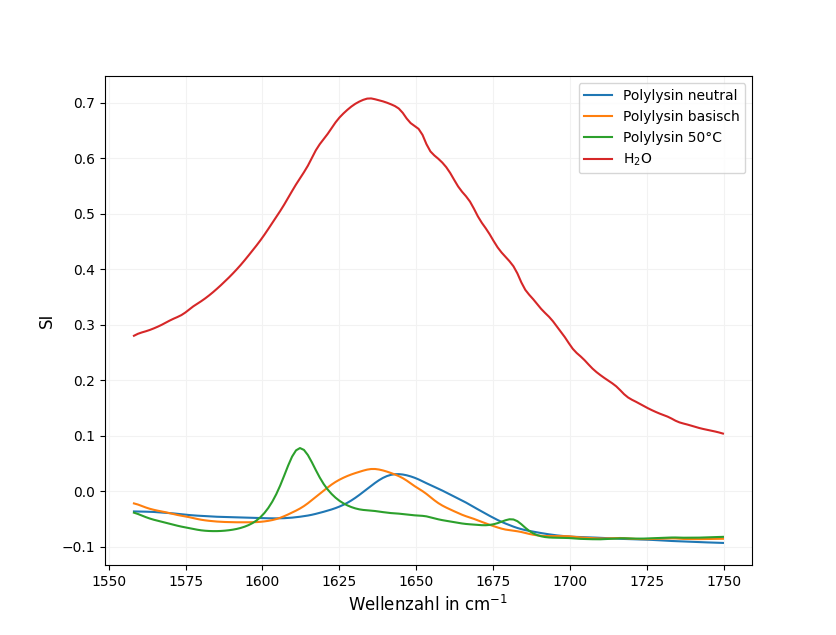
\includegraphics[scale=0.55]{water_polylysin.png}
				\caption{Infrarotspektrum von Wasser und Polylysin im Bereich von $\tilde{\nu}$ = 1550-1750 cm$^{-1}$}
				\label{fig:water_polylysin_full}
			\end{figure}
			
			Für Den vergleich Wasser und Deuteriumoxid und warum, welches geeigneter für eine Messung wäre, müsste die Messung wiederholt werden, da nicht nachvollzogen werden kann, welche Probe das "Deuteriumoxid"-Spektrum ist.
			
			\subsection{Citronensäure}
				Citronensäure ist ein Molekül das bei Ultra Violettes Licht ein breites Absorptionsbande im Bereich von $\lambda$ = 200 nm bildet \cite{Citricacid_UV}. Das ist für die heutigen Photometer kaum messbar, weswegen die IR-Spektroskopie eine gute Messmethode darstellt.\\
				Citronensäure zeigt eine intensive SI$_{max}$ im Bandenbereich von 1500 - 1800 cm$^{-1}$, welches geeignet ist für die quantitative Analyse von Citronensäure.\\
				Da sowohl Deuteriumoxid und Wasser in der Absorption diese Bande bei Citronensäure etwas überlappen, macht es kein Unterschied ob Citronensäure in Wasser oder in Deuteriumoxid gemessen wird. Da Deuterium teurer ist als Wasser und auch nicht zugänglicher ist, ist es wirtschaftlich sinnvoll Citronensäure in Wasser zu messen.\\
				Für die beiden unbekannten Proben 1 und 2wurde eine Konzentration von 1.04 $\pm$ 0.012 mM und 0.58 $\pm$ 0.007 gemessen.
				Da jeweils bei der Standardreihe und bei der Probe nur eine Einfachmessung durchgeführt wurde, weichen die Werte sehr von dem realen Wert ab.\\
				Für eine bessere quantitative Aussage sollen mehr Mehrfachwerte der einzelnen Proben durchgeführt werden. Außerdem soll auch die Messfehlern von den Geräten mitnotiert werden, für eine vollständige Fehleranalyse.\\
				Trotzalldem konnte gezeigt werden, dass mit IR-Spektroskopie auch eine quantitative und qualitative Untersuchung einer Probe möglich ist.
			
			
			\subsection{Polylysin}
				Die Amid I Bande, welches für die Sekunddärsturkturaufklärung die meiste Bedeutung hat, hat ihre Absorptionsbande im Bereich 1600 - 1700 cm$^{-1}$.
				Die für diesen Versuch verwendete Referenzwerten wurde in Table \ref{tab:ref_values_sec_stru} dargestellt.
					\begin{table}[H]
						\centering
						\caption{Bandenposition von Peptiden in Wasser der Amid I Bande\cite{Script}.}
						\label{tab:ref_values_sec_stru}
						\begin{tabular}{ccc}
							\toprule
							Sekundarstruktur & Average in  cm$^{-1}$& Extrema in cm$^{-1}$\\
							\midrule
							$\alpha$-Helix & 1652 & 1642 - 1660\\
							\midrule
							\multirow{2}{*}{ß-Faltblatt } & 1630 & 1615 - 1638\\
							& 1679 & 1672 - 1694\\
							\midrule
							Turns & 1671 & 1653 - 1692 \\
							\midrule
							Disordered & 1645 & 1639 - 1654\\
							\bottomrule
						\end{tabular}
					\end{table}				
						
			Polylysin in Deuteriumoxid bei neutralen pH hat ein Absorptionsmaxima in der Amid I Bande bei 1644 cm$^{-1}$ was nach der Table \ref{tab:ref_values_sec_stru} die $\alpha$-Helix Struktur ihren SI$_{max}$ zeigt.\\
			Polylysin im basischen Bereich hat ihren SI$_{max}$  bei 1636 cm$^{-1}$, dass nahelegt, dass es eine disordered Struktur zeigt.\\
			Beim Aufwärmen des Peptids auf 50°C bilden sich zwei SI$_{max}$  bei 1612 und 1680 cm$^{-1}$, welches im Bereich des ß-Faltblatt liegt.\\
			Es ist schwierig die disordered und $\alpha$-Helix Struktur auseinander zu halten, da die Bandenposition der beiden überlappen und die Peaks sehr nahe liegen. Zusätzlich sind die Referenzwerte in Table \ref{tab:ref_values_sec_stru} Messwerte von Peptiden in Wasser und nicht in  Deuteriumoxid.\\
			Nach Zhang et al\cite{Polylysin} zeigt Polylysin bei nicht basischen Bedingung eine disordered Konformation auf und bei basischen eine $\alpha$-Helix-Konformation.\\
			Um dieses bestätigen zu können, muss der Versuch nochmal wiederholt werden und die Proben auch in Wasser zu messen, um diese mit der Referenzwerten besser vergleichen zu können.
			Trotzalldem konnte gezeigt werden, dass die Sekundärstruktur ihre charakteristischen Absorptionsmaxima in der Amid I Bande besitzen und Polylysin gut geeignet ist, diese zu untersuchen.
			Die Konformationsänderung der Probe bei Bedingungsänderung konnte hier gut nachverfolgt werden.

		
	\section{Anhang}
		\subsection{Rohdaten}
		
			
			
			\begin{table}[H]
				\centering
				\caption{Signalintensitäts-Werte der Standardreihe.}
				\label{tab:r_square_standardcurve}
				\begin{tabular}{cc}
					\toprule
					c(Citronensäure) in mM & SI$_{max}$\\
					\midrule
					0.2	&0.035\\
					0.4	&0.074\\
					0.6	&0.109\\
					0.8	&0.146\\
					1.0	&0.159\\
					1.2	&0.188\\
					1.4	&0.226\\
					1.6	&0.258\\
					1.8	&0.295\\
					2.0	&0.327\\
					\bottomrule
				\end{tabular}
			\end{table}	
			
			\begin{figure}[H]
				\centering
				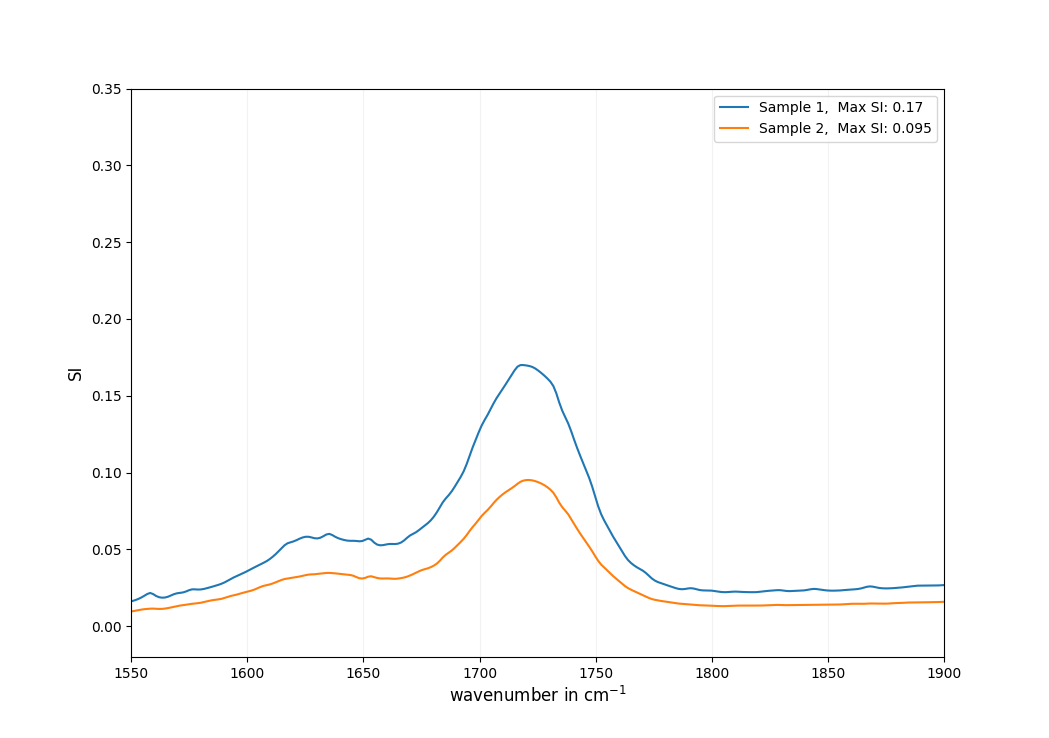
\includegraphics[scale=0.55]{unknown_sample.png}
				\caption{Infrarotspektrum der unbekannten Citronensäuren Proben.}
				\label{fig:IR_unknown}
			\end{figure}
				
			\begin{table}[H]
			\centering
			\caption{Signalintensitäts-Werte der unbekannten Citronensäure.}
			\label{tab: SI_unknownsample}
				\begin{tabular}{cc}
						\toprule
						Probe & SI$_{max}$\\
						\midrule
						Sample 1 & 0.170\\
						Sample 2 & 0.095\\
						\bottomrule
				\end{tabular}
			\end{table}			
		
			\begin{table}[H]
				\centering
				\caption{Pipettierschema der Standardreihe von Citronensäure in H$_2$O. Die molare Konzentration der Stammlösung beträgt 2mM in Wasser.}
				\label{tab:pipettierschema Standardreihe}
				\begin{tabular}{ccc}
					\toprule
					c(Citronensäure) in mM &V(2mM Citronensäure) in mL & V(H$_2$O in mL)\\
					\midrule
					2.0 & 2.0 & 0.0\\
					1.8 & 1.8 & 0.2\\
					1.6 & 1.6 & 0.4 \\
					1.4 & 1.4 & 0.6 \\
					1.2 & 1.2 & 0.8\\
					1.0 & 1.0 & 1.0 \\
					0.8 & 0.8 & 1.2\\
					0.6 & 0.6 & 1.4\\
					0.4 & 0.4 & 1.6 \\
					0.2 & 0.2 & 1.8 \\
					0.0 & 0.0 & 2.0\\
					\bottomrule
				\end{tabular}
			\end{table}	
	
	\addcontentsline{toc}{section}{References}
	\bibliographystyle{plainurl}
	\nocite{*}
	\bibliography{Literatur}
	\newpage
	
	
\end{document}